\chapter{Neural networks}
%
\index{Online character reorganization}
\index{Online character recognition}
\index{Offline character recognition}
Neural networks are our tool of choice for our implementation project.
We want to recognize mathematical expressions and also consider Kanji recognition.
Challenges for these applications are especially ambiguity of handwriting and implicit
conventions applied to notation. As a result, the quality of such applications
varies greatly.
This particular implementation cannot compete with industrial applications due to time constraints for this thesis.

Recognizing handwriting recorded with a digitizer as a time sequence of pen
coordinates is known as \emph{online character reorganization}.
As opposed to \emph{offline handwritten character recognition} dealing
with the scanned handwritten document~\cite{kumar2013offline}.
Our implementation only covers online recognition.

\section{Structure of neural networks}
%
The definitions in this chapter are based on Christopher M. Bishop's book \emph{Pattern Recognition and Machine Learning}~\cite{Bishop}.
In this thesis, we generally use the term \emph{Neural network} deliberately for the multilayer perceptron on page~227 ff. as a result of considerations of linear models.
The linear models deal with the following problems:

\begin{problem}[Regression problem]
  Given a training data comprising $N$ observations $\{x_n\}$, where $n = 1, \ldots, N$ together with corresponding target values $\{t_n\}$, the goal is to predict the value of $t$ for a new value of $x$.~\cite[p.~138]{Bishop}
\end{problem}
\begin{problem}[Classification problem]
  Take an input vector $x$ and assign it to one of $K$ discrete class $\mathcal C_k$ where $k = 1, \ldots, K$.~\cite[p.~179]{Bishop}
\end{problem}

The models are based on linear combinations of fixed nonlinear basis functions~$\varphi_j(x)$:
\begin{align}
  y(x, w) &= f\left(\sum_{j=1}^M w_j \varphi_j(x)\right)
\end{align}

In this case, $x$ represents the input vector, $w$ represents so-called \emph{weights}, $\varphi_j(x)$ denotes the $j$-th fixed nonlinear basis function and $f(\cdot)$ is a nonlinear activation function. In the case of regression, $f(\cdot)$ is the identity function.

\TODO{Explain layers}

\TODO{Discuss the properties of a neural network of two inputs, one hidden layer, and one output}

\section{Neural networks in practice}

\subsection{Curve Fitting Problem in Neural Networks}

\TODO{Illustrate the exercises given by Takayama-sensei}

\subsection{Backpropagation}

\TODO{Explain the algorithm}

\subsection{Gradient Descent}

Gradient Descent is an iterative optimization algorithm. It utilizes the gradient
of the function to minimize the function value. The method dates at least back to
Cauchy~\cite{cauchy-gd}, who used it for astronomical calculations.
In Machine Learning, we use Gradient
Descent for the error function

\TODO{Explain the algorithm and exercises}

\TODO{Give convergence proof}

\section{Google TensorFlow}
\label{sec:nn-tensorflow}
%
\index{Classification}
\index{Regression}
Google TensorFlow~\cite{abadi2016tensorflow} is an open-source software library for Machine Intelligence.
It provides users a choice between a high-level and a low-level API.
This enables them to implement a wide variety of Machine Learning applications.
We will list some basic application classes distinguished in Machine Learning:
\begin{description}
  \item[Supervised learning]
    labelled data is available used in training phase, validation possible
    \begin{description}
      \item[regression] output values are continuous
      \item[classification] output values are discrete
    \end{description}
  \item[Unsupervised learning]
    labelled data unavailable, validation impossible
    \begin{description}
      \item[clustering] find groups of similar features
      \item[density estimation] find distribution of data within input space
    \end{description}
\end{description}

For our application, TensorFlow is the tool of choice.
We used the Python API to implement our handwriting recognition system.

\section{Terminology}
\label{sec:nn-terminology}
%
A \emph{glyph} is a visual unit drawn on any surface visible to a potential reader.
A \emph{character} is the perceived unit of writing.
\emph{Unicode}~\cite{unicode} is an encoding covering most of the world's writing systems.
A \emph{Unicode code point} is a unique number assigned to a character.

\section{A problem statement}
\label{sec:problem-statement}
%
The problem of handwriting recognition dates back to the early days of machine learning even before 1960~\cite{5244320}.
Since the beginning, it was considered a more convenient and natural way to input text into a machine.
This is because most people learn to write with pen and paper before they learn to type text on a keyboard.
The requirement of a keyboard for typing is impractical for mobile applications.
Instead, the industry developed devices, where a pen or your finger is used as an input interface on a surface tracking your motion.
Handwriting recognition has gained attention on handheld devices such as personal digital assistants (PDA).
With the recent advent of smartphones after the year 2000, new input devices were used for handwriting.
The screens got large enough such that the user can draw the desired characters and applications recognize the glyphs.
Even though the quality has improved tremendously since the 1960s, most users still prefer a virtual keyboard over character drawing interfaces.

The MNIST dataset~\cite{lecun1998mnist} is the most famous dataset to begin an application with.
Extremely high accuracies have been obtained~\cite{surinta2015recognition} to recognize the digits given in this dataset.
However, there are many other datasets consisting of less examples and which can be considered more difficult.
The aforementioned paper~\cite{surinta2015recognition} considers Thai, Bangla, and Latin scripts, which employs new challenges considering a high variability in the shapes, strokes, curls, and concavities.

They collected a Thai handwritten script dataset containing 24,045 character images in total from various writers.
Figure~\ref{fig:tbl-examples} shows examples for the Thai, Bangla, and Latin scripts.
Recognize that the Bangla numeral 4 (Example b, row 2, column 5 in Figure~\ref{fig:tbl-examples}) and the Latin digit 8 (Example b, row 3, column 9) are written the same way.
It follows immediately that recognition software must not only recognize individual characters, but has to use context information to determine which script is used.
Accuracies above 95~\%, 88~\% and 60~\% for Latin, Thai, and Bangla scripts, respectively using support vector machines.

\begin{figure}[!h]
  \begin{center}
    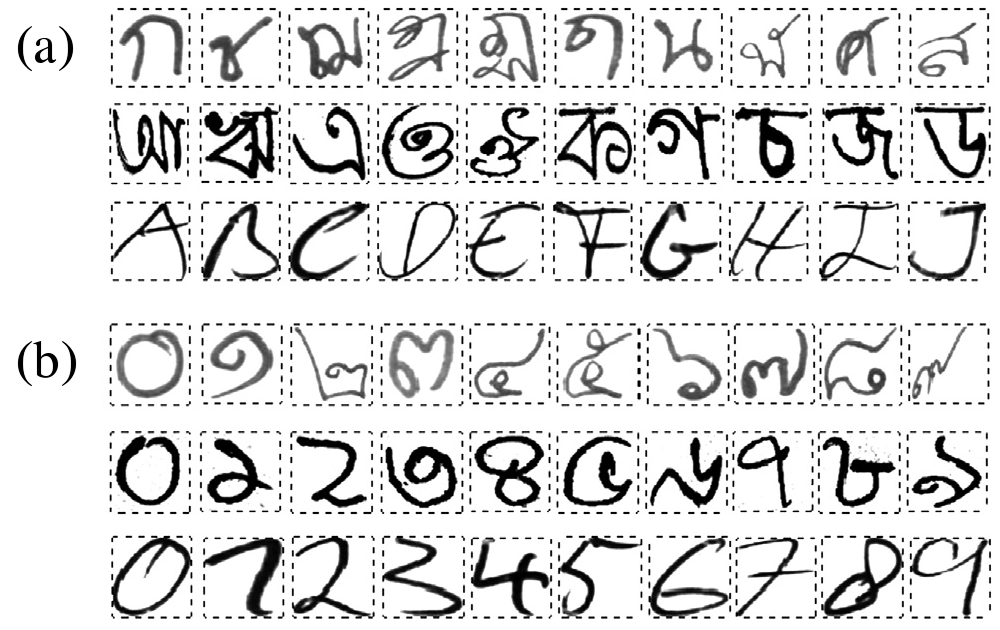
\includegraphics[width=0.8\textwidth]{img/thai-bangla-latin-handwriting.png}
    \caption{
      Thai, Bangla, and Latin handwriting example shown in the first, second and third row, respectively.
      Sample (a) shows handwritten characters and (b) shows handwritten digits.
    }
    \label{fig:tbl-examples}
  \end{center}
\end{figure}

In this thesis, we want to focus on two tasks. The first task is a generic version of the second task.
\begin{enumerate}
  \item Given the stroke traces of drawn characters, recognize the syntax and semantics of the characters and forward the data to a domain-specific application in an appropriate format.
  \item Given the stroke traces of mathematical characters, recognize the syntax and semantics of the characters and return its representation in mathematical notation formats such as \LaTeX{} or MathML~\cite{MathML}.
\end{enumerate}
has gained a lot of momentum since the increase of the Internet~\cite{chan2000mathematical}.


\TODO{Add the wonderful pathological examples mentioned in the papers, I read}

\section{Current state}
%
\TODO{Sum up the papers, you read}
\TODO{Show some existing implementations}

\section{Implementation}
\label{sec:implementation}
%
Our application implements 5 stages. Namely,
\begin{description}
\item[segmentation] splitting into individual characters,
\item[recognition] given a drawn character, return the corresponding Unicode point,
\item[annotation of spatial information] spatial relationship between characters is added,
\item[correction] using the context information, we apply corrections to the recognized characters,
\item[output format] we generate the desired MathML/\LaTeX{} output.
\end{description}

\subsection{Segmentation}
\label{sec:impl-segmentation}
%
We decided in favor of a very simple implementation for this step.
Every stroke is considered as individual character unless it intersects with another stroke.
Two or more intersecting strokes are considered as one character.
This unit is passed on to the next stage.

\subsection{Recognition}
\label{sec:impl-recognition}
%
First, we define the glyphs, we want to recognize. In general, mathematical notation can be intermingled with text,
but we restrict our recognition system to the latin script combined with mathematical symbols. This restriction might
be insufficient for other recognition applications. But the task to recognize text in languages such as Japanese, Arabic
and Hewbrew goes beyond the scope of the problem tackled in this thesis.

We define four properties:
\begin{enumerate}
\item We want to recognize mathematical symbols, latin script and numbers.
  We use Unicode points to reference these characters.
\item A character $X$ is \emph{visually similar} to another character $Y$,
  if at least one of the following conditions is met~\footnote{
    Visual similarity as defined above is a reflexive, symmetric and transitive binary relation (hence, an equivalence relation).
  }:
  \begin{itemize}
    \item if $X$ and $Y$ are commonly written in the same stroke layout by handwriters,
    \item $X$ is a larger version of $Y$ or vice versa,
    \item $X$ has the same layout like $Y$ and only distinguishes itself by the position within the character boundaries.
  \end{itemize}
\item We want to recognize most characters individually.
  Some characters are visually difficult to distinguish.
  Two or more visually similar glyphs are represented in a \emph{character group} (a set of Unicode points).
  We distinguish the characters later context-sensitively.
  \index{Character group}
\item A character group is represented by its \emph{representative} (one Unicode point),
  i.e. the member with the smallest Unicode point value.
  \index{Representative}
\end{enumerate}

In order to retrieve the list of character groups and representatives,
we using the following algorithm:
%
\begin{enumerate}
\item
  We consider
  \begin{itemize}
  \item the Latin alphabet of the Basic Latin block (U+0041-U+005A, U+0061-U+007A),
  \item the Mathematical Operators block (U+2200-U+22FF),
  \item the Supplemental Mathematical Operators block (U+2A00–U+2AFF),
  \item extended by Hindu-Arabic digits, and
  \item some more characters considered important for mathematical character recognition.
  \end{itemize}
  Our sources specify 706 Unicode points.
\item
  These characters are taken and Unicode-normalized~\cite{unicode-norm} using the form NFKD
  (decomposition by compatibility followed by recomposition respecting canonical equivalence).
  One exception is \usymrepr{⫝̸}{FORKING}. This character is not normalized (see below).
  The resulting characters from the normalization constitute our new list of Unicode points.
  8 characters get lost.
\item
  A custom list defines visually similar characters. Thus some characters are merged into
  the same character group. 648 Unicode point representatives are left.
\end{enumerate}

This process is required, because character properties such as size are relative.
Therefore we defined visual similarity, character classes and their representatives above.
Consider, for example, a glyph drawn to represent digit 2.
We cannot determine whether it corresponds to \usymrepr{2}{DIGIT TWO} or \usymrepr{${}_2$}{SUBSCRIPT TWO},
because size is only difference between the characters. Size vastly depends on the size of the drawing area.
As such we want to recognize both inputs as \usymrepr{2}{DIGIT TWO} and use context-sensitive information later on
to potentially replace it with unicode point \usymrepr{${}_2$}{SUBSCRIPT TWO}.
Unicode normalization provides us a standardized way to normalize the characters.

We want to illustrate this process with examples.
\begin{itemize}
  \item
    The character \usymrepr{A}{LATIN CAPITAL LETTER A} is passed through the whole algorithm
    and is added in its original form.
  \item
    The character \usymrepr{Ⅱ}{ROMAN NUMERAL TWO} is normalized to \usymrepr{II}{LATIN CAPITAL LETTER I, LATIN CAPITAL LETTER I}.
    Because these characters are equivalent to the existing individual symbol \usymrepr{I}{LATIN CAPITAL LETTER I},
    nothing is actually changed in the database by adding \usymrepr{Ⅱ}{ROMAN NUMERAL TWO}.
  \item
    However, \usymrepr{⫼}{LARGE TRIPLE VERTICAL BAR OPERATOR} is not decomposed into three individual code points.
  \item
    Sometimes the opposite process takes place. Character \usymrepr{⫝̸}{FORKING} is identified as one unicode point point.
    But normalization returns two characters.
    Namely, \usymrepr{⫝}{NONFORKING} and \usymrepr{/}{COMBINING LONG SOLIDUS OVERLAY}.
    This exception has been removed explicitly in step~2 of the algorithm above.
  \item
    The character \usymrepr{≝}{EQUAL TO BY DEFINITION} is a combination of the character \usymrepr{=}{EQUALS SIGN}
    and \usymrepr{def}{LATIN SMALL LETTER D, LATIN SMALL LETTER E, LATIN SMALL LETTER F}.
    Symbol \usymrepr{=}{EQUALS SIGN} itself is a composition of two characters \usymrepr{-}{HYPHEN-MINUS}.
    However, Unicode normalization retains the same character.
\end{itemize}

Because of this process, a hierarchical structure of glyph components is implied.
A glyph can be decomposed if two or more non-intersecting strokes are part of a glyph
and those strokes occur in at least one other glyph.

\TODO{describe stroke simplification algorithm}

\TODO{Describe the database we used to compare characters with}

\subsection{Annotation}
\label{sec:impl-annotation}
%
\TODO{describe how the spatial information is encoded}

\subsection{Correction}
\label{sec:impl-correction}
%
\TODO{describe how correction is done}
\TODO{HMM desired, but was too complex for this thesis}

\subsection{Output format}
\label{sec:impl-output}
%
\TODO{Show MathML/LaTeX example}
